%%%%%%%%%%%%%%%%%%%%%%%%%%%%%%%%%%%%%%%%%
% Quick Start Example
% 
% $Date$
% $Rev$:
% $Author$


\chapter{Quick Start Example}\label{chap:example}

This chapter provides a brief introduction to \Kieker{} based on a simple %
Bookstore example application. Section~\ref{sec:example:downloadInstall} %
explains how to download and install \Kieker{}. The Bookstore application itself %
is introduced in Section~\ref{sec:example:bookstore}, while the following %
sections and demonstrate %
how to use \Kieker{} for monitoring~(Section~\ref{sec:example:monitoring}) and %
analyzing~(Section~\ref{sec:example:analysis}) the resulting monitoring data. %

%%
\section{Download and Installation}\label{sec:example:downloadInstall}

The Kieker download site\footnote{\KiekerDownloadURL{}} provides archives %
of the binary and source distribution, the Javadoc~API, as well %
as additional examples. %The archives are available in tar.gz and zip format.
For this quick start guide the \Kieker{}'s binary distribution, e.g., %
\file{\binaryFileForDownload}, is required and must be downloaded. %
After having extracted the archive, you'll find the directory structure and %
contents shown in Figure~\ref{fig:binary-layout}.

% Note: The indention is not really necessary, but the tree is easier to understand in the tex-source.
\begin{figure}%[H]
\begin{graybox}
\dirtree{%  
	.1 \DirInDirTree{\KiekerDir/}.
		.2 \DirInDirTree{bin/}\DTcomment{Call scripts for \Kieker{} tools}. 
			.3 \ldots. 
		.2 \DirInDirTree{doc/}\DTcomment{}. 
			.3 \DirInDirTree{tutorial/}. 
				.4 userguide.pdf\DTcomment{PDF file of this document}. 
				.4 \DirInDirTree{\exampleDir/}\DTcomment{Source code of the examples in this document}. 
		.2 \DirInDirTree{dist/}\DTcomment{The \Kieker{} framework libraries}. 
			.3 \mainJar. 
			.3 \servletWar. 
		.2 \DirInDirTree{lib/}\DTcomment{Libraries required by \Kieker{}}. 
			.3 \commonsLoggingJar.
			.3 \ldots. 
		.2 \DirInDirTree{META-INF/}\DTcomment{Example configuration files}. 
			.3 \kiekerMonitoringProperties{}.
			.3 \ldots. 
}
\end{graybox}
\caption{Directory structure and contents of \Kieker{}'s binary distribution}
\label{fig:binary-layout}
\end{figure}

This document as well as the Java sources of the included examples %
can be found in the directory~\dir{\userGuideDir{}/}. %
The file \file{\mainJar{}} contains the \KiekerMonitoringPart{} and %
\KiekerAnalysisPart{} components, as well as the \KiekerTraceAnalysis{} tool. %
A Servlet-based Web application, provided in \file{\servletWar}, can be used %
to view and control the status of \KiekerMonitoringPart{} in Java~EE %
environments. The \file{\kiekerMonitoringProperties{}} is a sample configuration %
file for \KiekerMonitoringPart{}, as detailed in Chapter~\ref{chap:componentsMonitoring}. %
Since \Kieker{} uses the Apache Commons library~\cite{CommonsLogging-WebSite} %
as a logging interface, the file \file{\commonsLoggingJar} is the only dependency %
to a third-party library which is needed by \Kieker{} in every case. 

%%
\section{Bookstore Example Application}\label{sec:example:bookstore}

The Bookstore application is a small sample application resembling a simple %
bookstore with a marketplace facility where user can search for books in an %
online catalog and subsequently get offers from different book sellers. %
Figure~\ref{fig:bookstore:classAndSequenceDiagrams} shows %on the left side 
a class diagram describing the structure of the bookstore and %on the right side 
a sequence diagram illustrating the dynamics of the application. 

\begin{figure}[h]\centering
\subfigure[]{\label{fig:boostore:classdiagram}%
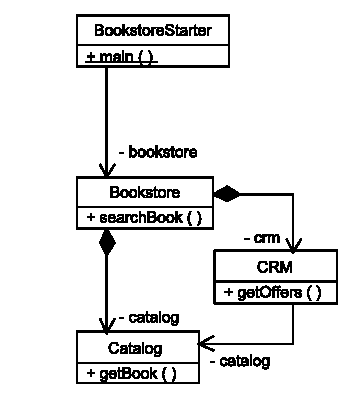
\includegraphics[scale=0.8]{images/kieker_bookstoreclassdiagram}%
}%
\subfigure[]{\label{fig:boostore:sequencediagram}%
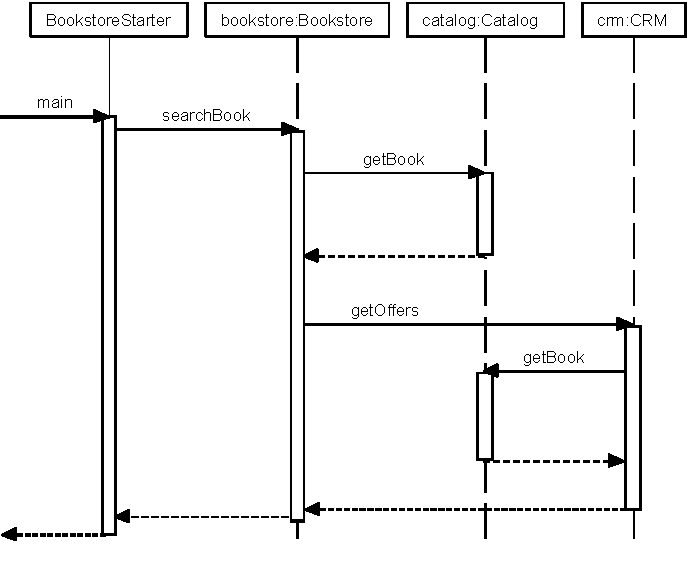
\includegraphics[scale=0.8]{images/kieker_SequenceDiagram-manually-changed}%
}
\caption{UML class diagram~\subref{fig:boostore:classdiagram} and %
sequence diagram~\subref{fig:boostore:sequencediagram} of the Bookstore application}
\label{fig:bookstore:classAndSequenceDiagrams}
\end{figure}

The bookstore contains a catalog for books and a customer relationship %
management system~(CRM) for the book sellers. To provide this service, the different classes %
provide operations to initialize the application, search for books and get offers %
for searched books. In this example, the methods implementing these operations are %
merely stubs. However, for the illustration of \Kieker{} they are sufficient and the %
inclined reader may extend the application into a real bookstore. 

The directory structure of the Bookstore example is shown in %
Figure~\ref{fig:PlainBookstoreExample} and comprises four Java classes in %
\dir{example/src/bookstoreApplication/} which are detailed below.

\begin{figure}[H]
\begin{graybox}
\dirtree{%
.1 \DirInDirTree{example/}. %\DTcomment{The root directory of the project}.
.2 \DirInDirTree{build/}\DTcomment{Directory for the Java class files}. 
.2 \DirInDirTree{src/}\DTcomment{The directory for the source code files}.
.3 \DirInDirTree{bookstoreApplication/}.
.4 Bookstore.java.
.4 BookstoreStarter.java.
.4 Catalog.java.
.4 CRM.java.  
}
\end{graybox}

\caption{The directory structure of the Bookstore application}
\label{fig:PlainBookstoreExample}
\end{figure}

\NOTIFYBOX{The Java sources of the uninstrumented bookstore described in this section %
can be found in the \file{\plainBookstoreApplicationDir{}/} directory.}

\quad\

\noindent The class \class{BookstoreStarter}, shown in Listing~\ref{lst:class:BookstoreStarter}, %
contains the application's \method{main} method, i.e., the program start routine. It initializes the \class{Bookstore} and issues five search requests by %
calling the \method{searchBook} method of the \object{bookstore} object.

\setJavaCodeListing

\lstinputlisting[caption=BookstoreStarter.java,label=lst:class:BookstoreStarter]{\plainBookstoreApplicationDir/src/bookstoreApplication/BookstoreStarter.java}

\noindent The \class{Bookstore}, shown in Listing~\ref{lst:class:Bookstore}, contains a catalog and a CRM object, representing the catalog of the bookstore and a customer relationship management system which can provide offers for books out of the catalog. The business method of the bookstore is \method{searchBook()} which will first check the catalog for books and then check for offers.

In a real application these methods would pass objects to ensure the results of the catalog search will be available to the offer collecting method. However, for our example we omitted such code. 

\lstinputlisting[caption=Bookstore.java,label=lst:class:Bookstore]{\plainBookstoreApplicationDir/src/bookstoreApplication/Bookstore.java}

\noindent The customer relationship management for this application is modeled in the \class{CRM} class shown in Listing~\ref{lst:class:CRM}. It only provides a business method to collect offers which uses the catalog for some lookup. The additional catalog lookup is later used to illustrate different traces in the application.

\lstinputlisting[caption=CRM.java,label=lst:class:CRM]{\plainBookstoreApplicationDir/src/bookstoreApplication/CRM.java}

\noindent The final class is \class{Catalog} shown in Listing~\ref{lst:class:Catalog}. It resembles the catalog component in the application.

\lstinputlisting[caption=Catalog.java,label=lst:class:Catalog]{\plainBookstoreApplicationDir/src/bookstoreApplication/Catalog.java}

\noindent After this brief introduction of the application and its implementation, the next step is to see the example running. To compile and run the example, the commands in Listing~\ref{lst:bookstoreStarterWin} can be executed. This document assumes that the reader entered the commands in the \dir{example/} directory.

\setBashListing
% \begin{lstlisting}
nils@Laptop:~/example/$ javac src/mySimpleKiekerExampleManual/*.java -d build

nils@Laptop:~/example/$ java -classpath ./build/:./lib/commons-logging-1.1.1.jar\
                        mySimpleKiekerExampleManual.BookstoreMonitoringStarter 
\end{lstlisting}
% \WARNBOX{The default command-line interpreter of Windows doesn't support automatic file expansion. Therefore every single sourcefile has to be passed:
\begin{lstlisting}[caption=Commands to compile and run the Bookstore application]
#\lstshellprompt{}# javac src/bookstoreApplication/Bookstore.java 
        src/bookstoreApplication/BookstoreStarter.java 
        src/bookstoreApplication/Catalog.java 
        src/bookstoreApplication/CRM.java 
        -d build/

#\lstshellprompt{}# java -classpath build/ bookstoreApplication.BookstoreStarter 
\end{lstlisting}
%
%}

\noindent The first command compiles the application and places the resulting four class files in the \dir{build/} directory. To verify the build process, the \dir{build/} directory can be inspected. The second command loads the bookstore application and produces the output shown in Listing~\ref{lst:result-noinstr}.

\begin{lstlisting}[caption=Example run of the ``plain'' application,label=lst:result-noinstr]
Bookstore.main: Starting request 0
Bookstore.main: Starting request 1
Bookstore.main: Starting request 2
Bookstore.main: Starting request 3
Bookstore.main: Starting request 4
\end{lstlisting}


\noindent In this section, the \Kieker{} example application was introduced and when everything went well, the bookstore is a runnable program. Furthermore, the composition of the application and its function should now be present. %
The next Section~\ref{sec:example:monitoring} will demonstrate how %
to monitor this example application employing \KiekerMonitoringPart{} using manual instrumentation.

%%
\section{Monitoring}\label{sec:example:monitoring}

In the previous Sections~\ref{sec:example:downloadInstall} and \ref{sec:example:bookstore}, the \Kieker{} installation and the example application have been introduced. In this section, the preparations for application monitoring, the instrumentation of the application, and the monitoring are explained.

\quad\

\WARNBOX{In this example, the instrumentation is done manually. %
This means that the monitoring probe is implemented by mixing monitoring logic %
with business logic, which is often not desired since the resulting code is %
hardly maintainable. \Kieker{} includes probes %
based on AOP (aspect-oriented programming, \cite{Kiczales1997}) %
technology, as covered by Chapter~\ref{chap:aspectJ}. However, to illustrate the %
instrumentation in detail, the quick start example uses manual instrumentation.}

The first step is to copy the \Kieker{} jar-file \file{\mainJar} to the \dir{lib/} directory of the example directory~(see Section~\ref{sec:example:bookstore}). The file is located in \dir{\KiekerDir/dist/} of the extracted \Kieker{} archive, as described in Section~\ref{sec:example:downloadInstall}. %
The file \file{\commonsLoggingJar} is located in \dir{\KiekerDir/lib/} directory and has to be copied to the \dir{lib/} directory of the example application. The final layout of the example directories is illustrated in Figure~\ref{fig:KiekerBookstoreExample}.

\begin{figure}[H]
\begin{graybox}
\dirtree{%
.1 \DirInDirTree{example/}. %\DTcomment{The root directory of the project}.
.2 \DirInDirTree{build/}\DTcomment{Directory for the Java class files}. 
.2 \newFileDirInDirTree{\DirInDirTree{lib/}}\DTcomment{Directory for the required libraries}.
.3 \newFileDirInDirTree{\mainJar}.
.3 \newFileDirInDirTree{\commonsLoggingJar}.
.2 \DirInDirTree{src/}\DTcomment{The directory for the source code files}.
.3 \ldots.
}
\end{graybox}
\caption{The directory structure of the Bookstore application with \Kieker{} libraries}
\label{fig:KiekerBookstoreExample}
\end{figure}

\NOTIFYBOX{The Java sources of the manually instrumented Bookstore application described in %
this section can be found in the \file{\manualInstrumentedBookstoreApplicationDir{}/} directory.}

\quad\

\noindent \Kieker{} maintains monitoring data as  so-called monitoring records. %
Section~\ref{sec:componentsMonitoring:monitoringRecords} describes how to define and use custom monitoring record types. %
The monitoring record type used in this example is an \textit{operation execution record} which %
is included in the \Kieker{} distribution. %
Figure~\ref{fig:OperationExecutionRecordClassDiagram} shows the %
attributes which  are relevant to this example. %
The record type will be detailed in Chapter~\ref{chap:aspectJ} .

\begin{figure}[H]
\begin{centering}
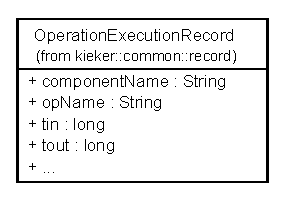
\includegraphics[scale=1]{images/kieker_OperationExecutionRecord-notraceattributes}%
\caption{The class diagram of the operation execution record}
\label{fig:OperationExecutionRecordClassDiagram}
\end{centering}
\end{figure}

\noindent The important attributes for the quick start guide are:

\begin{itemize}
\item[\hskip1em\class{componentName:}] In this case, the name of the class %
providing the called method
\item[\hskip1em\class{opName:}] The name of the called method
% \item traceId: The trace id of the current trace we want to record. Due to the fact, that we follow only one trace, this is zero in all recordings.
\item[\hskip1em\class{tin:}] The timestamp before calling the method
\item[\hskip1em\class{tout:}] The timestamp after the method returned
\end{itemize}

\noindent Listing~\ref{lst:cuttingBookstore} shows the instrumentation of the \class{Bookstore} class and its method \method{searchBook()}. In the lines 11 and 12, the monitoring controller is instantiated. It provides the monitoring service for the instrumentation.

% \TODO{Imports?!\\ --- avh: ja, evtl. mit linerange, aber er bl\"oderweise nummeriert er so durch}
% Make sure that this listing will be modified, once the sourcecode changes!!!
% It must show the whole monitoring of the bookstorecall, from getting the first time to persisting of the record!!

\setJavaCodeListing
\lstinputlisting[linerange={11-29}, firstnumber=11, caption=Instrumentation of the \method{getBook()} call in Bookstore.java, label=lst:cuttingBookstore]%
{\manualInstrumentedBookstoreApplicationDir/src/bookstoreApplication/Bookstore.java}
 
\noindent The lines 17 and 19 are used to determine the current time in nanoseconds before and after the \method{getBook()} call. In lines 20 to 23, a monitoring record for this measurement is created and initialized with the two time values. Additionally, the record has an attribute for the involved class \verb!Catalog! and the called method \method{getBook()}. Finally the record is handed over to the monitoring controller which calls a monitoring writer to persist the record. %
In this example, the filesystem writer is used---\Kieker{} uses this writer by default when no other writer is specified, %
as detailed in Section~\ref{sec:monitoring-log-writers}. %.

In addition to the instrumentation in the \class{Bookstore} class, the \method{getOffers()} method of the \class{CRM} class is instrumented as well. Similar to Listing~\ref{lst:cuttingBookstore}, measurements are taken before and after the call of the \object{catalog}'s \method{getBook()} method, as shown in %
lines~19 and~21 of Listing~\ref{lst:cuttingCRM}. Not shown in the listing is the instantiation of the monitoring controller. However, it is done in the same way as illustrated in Listing~\ref{lst:cuttingBookstore}. %And the complete example files can be found in the samples directory.
Finally, a record is created (see lines 22--25) and stored by calling the monitoring controller (see line 26).

\setJavaCodeListing
\lstinputlisting[firstline=16, firstnumber=16, lastline=27, caption=Instrumentation of the \method{getBook()} call in CRM.java, label=lst:cuttingCRM]%
{\manualInstrumentedBookstoreApplicationDir/src/bookstoreApplication/CRM.java}

\noindent %
The next step after instrumenting the code is running the instrumented application. Listing~\ref{lst:bookstoreStarterLinux} shows the two commands to compile and run the application in Linux or any other Unix-like system. Listing \ref{lst:bookstoreStarterWin} shows the same commands for Windows.

\setBashListing 		
\begin{lstlisting}
nils@Laptop:~/example$ javac src/mySimpleKiekerExampleManual/*.java\
 -classpath ./lib/°\commonJar°:./lib/°\monitoringJar°:\
 -d build

nils@Laptop:~/example$ java\
-classpath ./build/:\
./lib/°\commonJar°:./lib/°\monitoringJar°:./lib/°\commonsLoggingJar°\
mySimpleKiekerExampleManual.BookstoreMonitoringStarter 
\end{lstlisting}
	

\begin{lstlisting}[caption=Commands to compile and run the instrumented Bookstore under Windows,label=lst:bookstoreStarterWin]
#\lstshellprompt{}# mkdir build
#\lstshellprompt{}# javac src\bookstoreApplication\*.java -classpath lib\#\mainJar# -d build\

#\lstshellprompt{}# java -classpath build\;
       lib\#\mainJar#;
       lib\#\commonsLoggingJar#
       bookstoreApplication.BookstoreStarter 
\end{lstlisting}


\quad\

\WARNBOX{%
Windows' default command-line interpreter doesn't support automatic %
file expansion. Therefore every single source file has to be passed, as %
shown in Listing~\ref{lst:bookstoreStarterWin}. %
Also, it is necessary to separate the classpath elements by %
a semicolon instead of a colon.}

\quad\

\noindent If everything worked correctly, a new directory for the monitoring data with the name \dir{tpmon-20100727-181422131-UTC/} is created in the default temporary directory (see Listing \ref{fig:logtree}). The numbers in the directory name represent the time and date of the monitoring. Thus, they will be different numbers for every run.

\begin{figure}[H]
\begin{graybox}
\dirtree{%
.1 \DirInDirTree{/tmp/}.
.2 \DirInDirTree{tpmon-20100727-181422131-UTC/}.
.3 tpmon.map.
.3 tpmon-20100727-181422234-UTC-Thread-2.dat.
}
\end{graybox}
\caption{Directory structure after a monitoring run}
\label{fig:logtree}
\end{figure}

\noindent In \Kieker's default configuration, the log directory can be found in the default temporary directory: \dir{/tmp/} under \UnixLikeSystems{} and \dir{C:\textbackslash{}temp\textbackslash{}} under Windows. The monitoring directory contains two types of files. Files with the extension \dir{.dat} containing text representations of the monitoring records and a single file named \dir{tpmon.map} which contains information on the types of the monitoring records used. 

The Listings~\ref{lst:exampledat} and \ref{lst:examplemap} show example file contents. The \file{.dat}-file is saved in CSV format (\textbf{C}omma \textbf{S}eparated \textbf{V}alues)---in this case, the values of a monitoring record are separated by semicolons. To understand the \file{.dat}-file structure the semantics have to be explained. For this quick start example only some of the values are relevant. The first value \verb!$1! indicates the record type. The forth value indicates the class and method which has been called. And the seventh and eighth value are the start and end time of the execution of the called method.

\setBashListing
\lstinputlisting[caption=tpmon-20100727-181422234-UTC-Thread-2.dat (excerpt), firstline=1, lastline=3, label=lst:exampledat]%
{ch2-quickstart-example/tpmon-20100727-181422131-UTC/tpmon-20100727-181422234-UTC-Thread-2.dat}

\noindent The second file is a simple mapping file referencing keys to monitoring record types. In Listing~\ref{lst:examplemap} the key \verb!$1! is mapped to the type of operation execution records which were used in the monitoring. The key value corresponds to the key values in the \file{.dat}-file.

\lstinputlisting[caption=tpmon.map, label=lst:examplemap]%
{ch2-quickstart-example/tpmon-20100727-181422131-UTC/tpmon.map}

\noindent By the end of this section, two classes have been manually instrumented and at least one run of the instrumented application has been performed. As the recorded data can be viewed in spreadsheets or other applications which can process CSV-files, the next task is to use the \KiekerAnalysisPart{}-package as a sophisticated monitoring data analyzer. 

%%
\section{Analysis}\label{sec:example:analysis}

The last task of a successful application monitoring is the analysis of the collected information. In this section the data recorded in the monitoring task of the previous section is analyzed with the \KiekerAnalysisPart{}-package. At first the \Kieker{}-analysis library has to be added to the example. The second step is to write a suitable analyzer. And finally the analyzer is used to aggregate the information in a sensible way.

For this quick example guide, the analysis tool is very simple and does not show the full potential of \Kieker{}. For more detail read Chapter~\ref{chap:aspectJ} which uses the trace analysis tool of the \Kieker{}-package.

\begin{figure}[H]
\begin{graybox}
\dirtree{%  
.1 \DirInDirTree{example/}. 
.2 \DirInDirTree{build/}\DTcomment{Directory for the Java class files}. 
.2 \DirInDirTree{lib/}\DTcomment{Directory for the required libraries}.
.3 \ldots. 
.3 \mainJar.
.2 \DirInDirTree{src/}\DTcomment{The directory for the source code files}.
.3 \DirInDirTree{bookstoreApplication/}.
.4 \ldots. 
.4 \newFileDirInDirTree{BookstoreAnalysisStarter.java}.
.4 \newFileDirInDirTree{Consumer.java}.
}
\end{graybox}
\caption{Directory layout of the example application with the analysis files highlighted}
\label{lst:analysisExampleLayout}
\end{figure}

\noindent The analysis application itself comprises the files \file{Consumer.java} and \file{BookstoreAnalysisStarter.java} (as shown in Figure~\ref{lst:analysisExampleLayout}) which can be found in the example directory. 

Listing \ref{lst:Consumer} shows the content of the \file{Consumer.java} file which implements the \class{IMonitoringRecordConsumerPlugin} interface. This is the standard interface for the consumer of \Kieker{}-monitoring-records. If the term consumer is unclear at this point, please read Section~\ref{sec:kieker}.

\setJavaCodeListing       

\lstinputlisting[caption=Consumer.java, label=lst:Consumer]{\manualInstrumentedBookstoreApplicationDir/src/bookstoreApplication/Consumer.java}

\noindent The herein described consumer checks if each call of the \method{getBook()} method responded inside the given time boundaries. Meaning the maximal response time has not been exceeded. The maximal response time is set at instantiation of the \class{Consumer} class (see lines 14--16). 

For the data evaluation the \method{newMonitoringRecord()} (see lines 24--41) is used. This method is called for every monitoring record. At first the method tests if the monitoring record are really \class{OperationExecutionRecord} instances, as these are the only record types it can process. Then the methods calculates the execution time of one recorded \method{getBook()} call. If the method call takes longer than specified, a message is written directly to the error stream.

The methods \method{terminate} and \method{execute} don't do anything due to the fact that this consumer does not need any initialization. If the consumer would for example use threads then these methods would be the correct location to start and stop them.

After implementing a consumer, the application's main class has to be created. In this case the main program is located in the \file{BookstoreAnalysisStarter.java} file shown in Listing~\ref{lst:BookstoreAnalysisStarter}.

\setJavaCodeListing       
\lstinputlisting[caption=BookstoreAnalysisStarter.java,label=lst:BookstoreAnalysisStarter]{\manualInstrumentedBookstoreApplicationDir/src/bookstoreApplication/BookstoreAnalysisStarter.java}

\noindent The \class{BookstoreAnalysisStarter} follows a simple scheme. Each analysis tool has to create at least one \class{AnalysisInstance} which can be seen in Listing~\ref{lst:BookstoreAnalysisStarter} in line 19. Then the consumers are registered with the analysis instance. In this case the previously described \class{Consumer} is instantiated and the maximal response time is set to 3 nanoseconds. 

After preparing the analysis itself, the in- and outputs have to be set. This is done in line 24 were the output directory is set. Line 26 initializes an array of input directories. In this example the output directory is also used as an input directory. This might not be too wise in a real application. However, for this example it will suffice. In the next line (line 27) the log reader of the analysis instance is set. In this particular case a file system reader is used.

To set the whole analysis in motion, the analysis instance has to be started. This is done in line 30 of Listing~\ref{lst:BookstoreAnalysisStarter}.

As it can be seen, the application expects the output directory from the earlier monitoring run (see Section~\ref{sec:example:monitoring}) as argument, which must be passed manually. 

The Listings~\ref{lst:bookstoreAnalysisStarterLinux} and \ref{lst:bookstoreAnalysisStarterWin} describe how the analysis application can be compiled and run under Linux or other Unix-like systems and Windows.

\setBashListing 		

\begin{lstlisting}[caption=Commands to compile and run the analysis under \UnixLikeSystems{},label=lst:bookstoreAnalysisStarterLinux] 			
#\lstshellprompt{}# mkdir build
#\lstshellprompt{}# javac src/kieker/examples/userguide/ch2bookstore/manual/*.java 
        -classpath lib/#\mainJarEMF# -d build/

#\lstshellprompt{}# java -classpath build/:lib/#\mainJarEMF#
       kieker.examples.userguide.ch2bookstore.manual.BookstoreAnalysisStarter 
       /tmp/kieker-20120402-163314855-UTC-myHost-KIEKER-SINGLETON
\end{lstlisting}		
\begin{lstlisting}[caption=Commands to compile and run the analysis under Windows,label=lst:bookstoreAnalysisStarterWin]
#\lstshellprompt{}# mkdir build
#\lstshellprompt{}# javac src\kieker\examples\userguide\ch2bookstore\manual\*.java 
        -classpath lib\#\mainJarEMF# -d build\

#\lstshellprompt{}# java -classpath build\;lib\#\mainJarEMF#
       kieker.examples.userguide.ch2bookstore.manual.BookstoreAnalysisStarter 
       C:\Temp\kieker-20130910-120352847-UTC-myHost-KIEKER-SINGLETON
\end{lstlisting}	

	

It should be ensured that the application gets the correct path from the monitoring run. 

If everything worked correctly, the consumer should write something on the output stream for every record it gets. A possible display of the run can be found in the appendix of this tutorial. 
